\documentclass{standalone}
\usepackage{tikz}
\usetikzlibrary{patterns, positioning}


\begin{document}
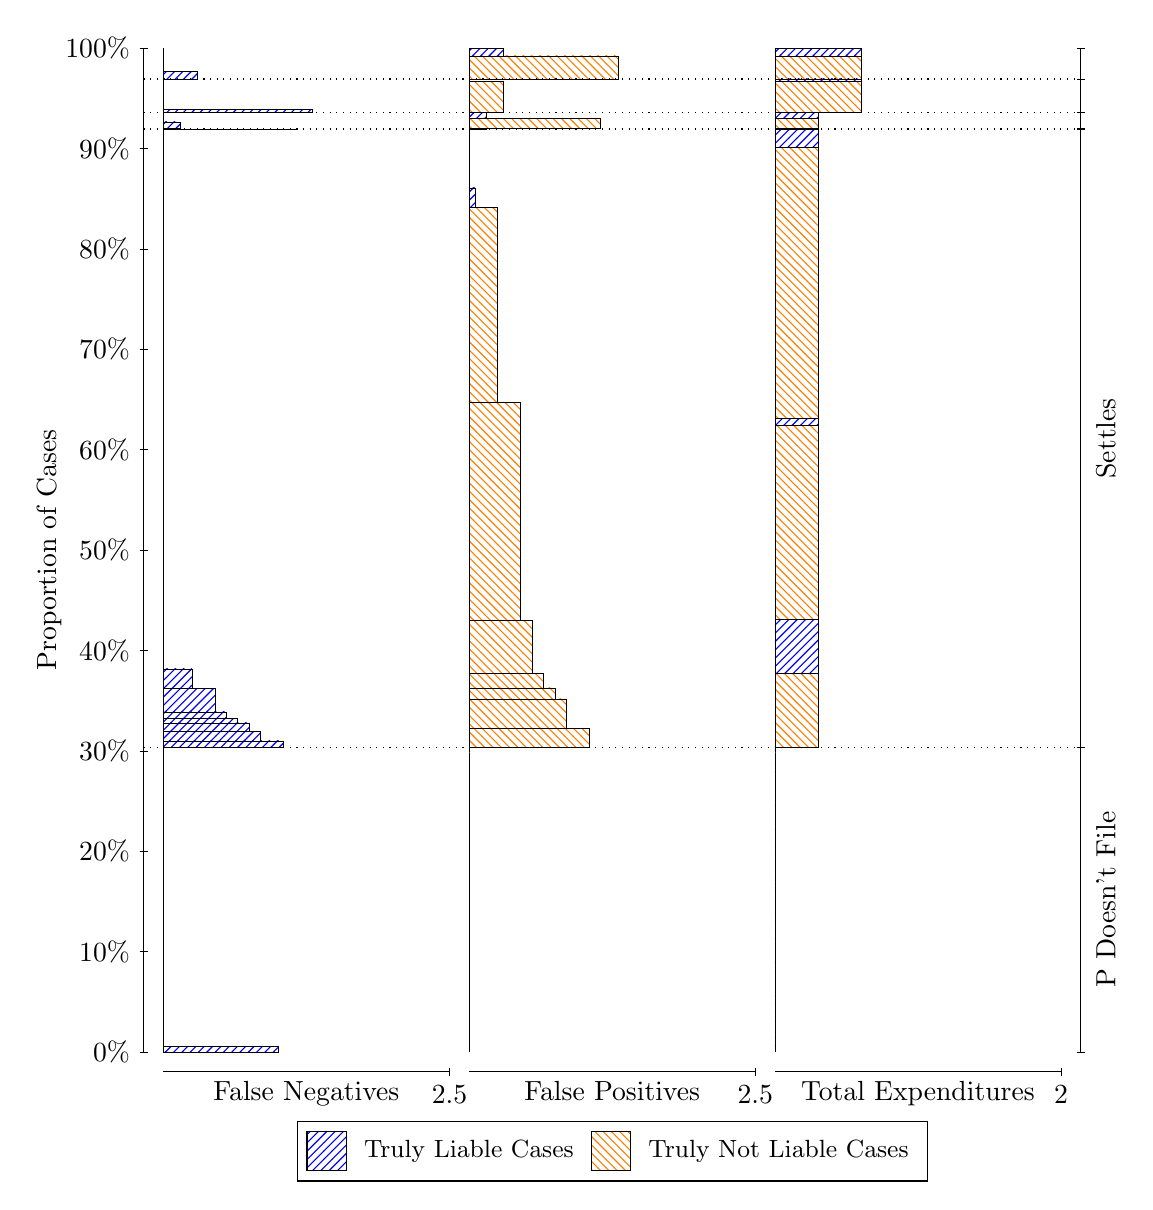
\begin{tikzpicture}
\draw[black, very thin] (1.5,1.75) -- (1.5,14.5);
\node[rotate=90, text=black, anchor=center] at (0.3, 8.125) {Proportion of Cases};
\draw[black, very thin] (1.45,1.75) -- (1.55,1.75);
\node[text=black, anchor=east] at (1.45, 1.75) {0\%};
\draw[black, very thin] (1.45,3.025) -- (1.55,3.025);
\node[text=black, anchor=east] at (1.45, 3.025) {10\%};
\draw[black, very thin] (1.45,4.3) -- (1.55,4.3);
\node[text=black, anchor=east] at (1.45, 4.3) {20\%};
\draw[black, very thin] (1.45,5.575) -- (1.55,5.575);
\node[text=black, anchor=east] at (1.45, 5.575) {30\%};
\draw[black, very thin] (1.45,6.85) -- (1.55,6.85);
\node[text=black, anchor=east] at (1.45, 6.85) {40\%};
\draw[black, very thin] (1.45,8.125) -- (1.55,8.125);
\node[text=black, anchor=east] at (1.45, 8.125) {50\%};
\draw[black, very thin] (1.45,9.4) -- (1.55,9.4);
\node[text=black, anchor=east] at (1.45, 9.4) {60\%};
\draw[black, very thin] (1.45,10.675) -- (1.55,10.675);
\node[text=black, anchor=east] at (1.45, 10.675) {70\%};
\draw[black, very thin] (1.45,11.95) -- (1.55,11.95);
\node[text=black, anchor=east] at (1.45, 11.95) {80\%};
\draw[black, very thin] (1.45,13.225) -- (1.55,13.225);
\node[text=black, anchor=east] at (1.45, 13.225) {90\%};
\draw[black, very thin] (1.45,14.5) -- (1.55,14.5);
\node[text=black, anchor=east] at (1.45, 14.5) {100\%};

\draw[black, very thin] (13.4,1.75) -- (13.4,14.5);
\draw[black, very thin] (13.35,1.75) -- (13.45,1.75);
\node[anchor=west] at (13.35, 1.75) {};
\draw[black, very thin] (13.35,5.6218) -- (13.45,5.6218);
\node[anchor=west] at (13.35, 5.6218) {};
\draw[black, very thin] (13.35,13.464) -- (13.45,13.464);
\node[anchor=west] at (13.35, 13.464) {};
\draw[black, very thin] (13.35,13.481) -- (13.45,13.481);
\node[anchor=west] at (13.35, 13.481) {};
\draw[black, very thin] (13.35,13.686) -- (13.45,13.686);
\node[anchor=west] at (13.35, 13.686) {};
\draw[black, very thin] (13.35,14.107) -- (13.45,14.107);
\node[anchor=west] at (13.35, 14.107) {};
\draw[black, very thin] (13.35,14.5) -- (13.45,14.5);
\node[anchor=west] at (13.35, 14.5) {};

\draw[black, very thin, pattern color=blue, pattern=north east lines] (1.75,1.75) rectangle (3.2033,1.8187);
\draw[black, very thin, pattern color=orange, pattern=north west lines] (1.75,1.8187) rectangle (1.75,5.6218);
\draw[black, very thin, pattern color=blue, pattern=north east lines] (1.75,5.6218) rectangle (3.276,5.7013);
\draw[black, very thin, pattern color=blue, pattern=north east lines] (1.75,5.7013) rectangle (2.9853,5.8178);
\draw[black, very thin, pattern color=blue, pattern=north east lines] (1.75,5.8178) rectangle (2.84,5.9303);
\draw[black, very thin, pattern color=blue, pattern=north east lines] (1.75,5.9303) rectangle (2.6947,5.9834);
\draw[black, very thin, pattern color=blue, pattern=north east lines] (1.75,5.9834) rectangle (2.5493,6.0686);
\draw[black, very thin, pattern color=blue, pattern=north east lines] (1.75,6.0686) rectangle (2.404,6.3631);
\draw[black, very thin, pattern color=blue, pattern=north east lines] (1.75,6.3631) rectangle (2.1133,6.614);
\draw[black, very thin, pattern color=orange, pattern=north west lines] (1.75,6.614) rectangle (1.75,13.464);
\draw[black, very thin, pattern color=blue, pattern=north east lines] (1.75,13.464) rectangle (3.4213,13.465);
\draw[black, very thin, pattern color=orange, pattern=north west lines] (1.75,13.465) rectangle (1.75,13.481);
\draw[black, very thin, pattern color=blue, pattern=north east lines] (1.75,13.481) rectangle (1.968,13.563);
\draw[black, very thin, pattern color=orange, pattern=north west lines] (1.75,13.563) rectangle (1.75,13.686);
\draw[black, very thin, pattern color=blue, pattern=north east lines] (1.75,13.686) rectangle (3.6393,13.718);
\draw[black, very thin, pattern color=orange, pattern=north west lines] (1.75,13.718) rectangle (1.75,14.107);
\draw[black, very thin, pattern color=blue, pattern=north east lines] (1.75,14.107) rectangle (2.186,14.205);
\draw[black, very thin, pattern color=orange, pattern=north west lines] (1.75,14.205) rectangle (1.75,14.5);
\draw[black, very thin, pattern color=orange, pattern=north west lines] (5.6333,1.75) rectangle (5.6333,5.5531);
\draw[black, very thin, pattern color=blue, pattern=north east lines] (5.6333,5.5531) rectangle (5.6333,5.6218);
\draw[black, very thin, pattern color=orange, pattern=north west lines] (5.6333,5.6218) rectangle (7.1593,5.8642);
\draw[black, very thin, pattern color=orange, pattern=north west lines] (5.6333,5.8642) rectangle (6.8687,6.2338);
\draw[black, very thin, pattern color=orange, pattern=north west lines] (5.6333,6.2338) rectangle (6.7233,6.3736);
\draw[black, very thin, pattern color=orange, pattern=north west lines] (5.6333,6.3736) rectangle (6.578,6.5579);
\draw[black, very thin, pattern color=orange, pattern=north west lines] (5.6333,6.5579) rectangle (6.4327,7.2302);
\draw[black, very thin, pattern color=orange, pattern=north west lines] (5.6333,7.2302) rectangle (6.2873,9.9993);
\draw[black, very thin, pattern color=orange, pattern=north west lines] (5.6333,9.9993) rectangle (5.9967,12.472);
\draw[black, very thin, pattern color=blue, pattern=north east lines] (5.6333,12.472) rectangle (5.706,12.723);
\draw[black, very thin, pattern color=blue, pattern=north east lines] (5.6333,12.723) rectangle (5.6333,13.464);
\draw[black, very thin, pattern color=orange, pattern=north west lines] (5.6333,13.464) rectangle (5.8513,13.48);
\draw[black, very thin, pattern color=blue, pattern=north east lines] (5.6333,13.48) rectangle (5.6333,13.481);
\draw[black, very thin, pattern color=orange, pattern=north west lines] (5.6333,13.481) rectangle (7.3047,13.603);
\draw[black, very thin, pattern color=blue, pattern=north east lines] (5.6333,13.603) rectangle (5.8513,13.686);
\draw[black, very thin, pattern color=orange, pattern=north west lines] (5.6333,13.686) rectangle (6.0693,14.074);
\draw[black, very thin, pattern color=blue, pattern=north east lines] (5.6333,14.074) rectangle (5.6333,14.107);
\draw[black, very thin, pattern color=orange, pattern=north west lines] (5.6333,14.107) rectangle (7.5227,14.401);
\draw[black, very thin, pattern color=blue, pattern=north east lines] (5.6333,14.401) rectangle (6.0693,14.5);
\draw[black, very thin, pattern color=orange, pattern=north west lines] (9.5167,1.75) rectangle (9.5167,5.5531);
\draw[black, very thin, pattern color=blue, pattern=north east lines] (9.5167,5.5531) rectangle (9.5167,5.6218);
\draw[black, very thin, pattern color=orange, pattern=north west lines] (9.5167,5.6218) rectangle (10.062,6.5579);
\draw[black, very thin, pattern color=blue, pattern=north east lines] (9.5167,6.5579) rectangle (10.062,7.2417);
\draw[black, very thin, pattern color=orange, pattern=north west lines] (9.5167,7.2417) rectangle (10.062,9.7145);
\draw[black, very thin, pattern color=blue, pattern=north east lines] (9.5167,9.7145) rectangle (10.062,9.794);
\draw[black, very thin, pattern color=orange, pattern=north west lines] (9.5167,9.794) rectangle (10.062,13.235);
\draw[black, very thin, pattern color=blue, pattern=north east lines] (9.5167,13.235) rectangle (10.062,13.464);
\draw[black, very thin, pattern color=orange, pattern=north west lines] (9.5167,13.464) rectangle (10.062,13.48);
\draw[black, very thin, pattern color=blue, pattern=north east lines] (9.5167,13.48) rectangle (10.062,13.481);
\draw[black, very thin, pattern color=orange, pattern=north west lines] (9.5167,13.481) rectangle (10.062,13.603);
\draw[black, very thin, pattern color=blue, pattern=north east lines] (9.5167,13.603) rectangle (10.062,13.686);
\draw[black, very thin, pattern color=orange, pattern=north west lines] (9.5167,13.686) rectangle (10.607,14.074);
\draw[black, very thin, pattern color=blue, pattern=north east lines] (9.5167,14.074) rectangle (10.607,14.107);
\draw[black, very thin, pattern color=orange, pattern=north west lines] (9.5167,14.107) rectangle (10.607,14.401);
\draw[black, very thin, pattern color=blue, pattern=north east lines] (9.5167,14.401) rectangle (10.607,14.5);
\draw[black, dotted] (1.5,5.6218) -- (13.4,5.6218);
\draw[black, dotted] (1.5,13.464) -- (13.4,13.464);
\draw[black, dotted] (1.5,13.481) -- (13.4,13.481);
\draw[black, dotted] (1.5,13.686) -- (13.4,13.686);
\draw[black, dotted] (1.5,14.107) -- (13.4,14.107);
\draw[black, very thin] (1.75,1.5) -- (5.3833,1.5);
\node[text=black, anchor=north] at (3.5667, 1.5) {False Negatives};
\draw[black, very thin] (5.3833,1.45) -- (5.3833,1.55);
\node[text=black, anchor=north] at (5.3833, 1.45) {2.5};

\draw[black, very thin] (5.6333,1.5) -- (9.2667,1.5);
\node[text=black, anchor=north] at (7.45, 1.5) {False Positives};
\draw[black, very thin] (9.2667,1.45) -- (9.2667,1.55);
\node[text=black, anchor=north] at (9.2667, 1.45) {2.5};

\draw[black, very thin] (9.5167,1.5) -- (13.15,1.5);
\node[text=black, anchor=north] at (11.333, 1.5) {Total Expenditures};
\draw[black, very thin] (13.15,1.45) -- (13.15,1.55);
\node[text=black, anchor=north] at (13.15, 1.45) {2};

\node[text=black, centered, rotate=90] at (13.72, 3.6859) {P Doesn't File};
\node[text=black, centered, rotate=90] at (13.72, 9.5431) {Settles};





\draw (7.449999999999999,1.5) node[draw=none] (baseCoordinate) {};
\begin{scope}[align=center]
        \matrix[scale=0.5, draw=black, below=0.5cm of baseCoordinate, nodes={draw}, column sep=0.1cm]{
            \node[rectangle, draw, minimum width=0.5cm, minimum height=0.5cm, pattern color=blue, pattern=north east lines] {}; &
            \node[draw=none, font=\small, text=black] (B) {Truly Liable Cases}; &
            \node[rectangle, draw, minimum width=0.5cm, minimum height=0.5cm, pattern color=orange, pattern=north west lines] {}; &
            \node[draw=none, font=\small, text=black] (B) {Truly Not Liable Cases}; \\
            };
\end{scope}

\end{tikzpicture}
\end{document}